\chapter{Triển khai thực nghiệm và đánh giá}
\label{Chapter5}

Chương này trình bày cách Yoca được triển khai thành một hệ thống hoàn chỉnh, từ môi trường vận hành và quy trình tích hợp mã nguồn đến các chức năng người dùng và kết quả kiểm thử. Nội dung được tổ chức theo hành trình sử dụng của sản phẩm, qua đó cho thấy mối liên hệ giữa dữ liệu thị trường, token, pool, ví, cảnh báo và các mô-đun hỗ trợ phân tích.

\section{Môi trường, tích hợp và triển khai hệ thống}
\label{sec:moi_truong_trien_khai}

Yoca là một ứng dụng web full-stack được tổ chức trong npm workspace. Client sử dụng React 19 và Vite 7 để xây dựng giao diện; server vận hành trên Node.js với Hono để xử lý xác thực, nghiệp vụ và tích hợp dịch vụ. PostgreSQL lưu dữ liệu tài khoản, cấu hình người dùng và các cache bền vững; Drizzle ORM quản lý lược đồ cùng các truy vấn liên quan. ECharts đảm nhiệm phần lớn biểu đồ tài chính, trong khi quan hệ giao dịch giữa các ví được biểu diễn bằng đồ thị tương tác.

Dữ liệu được phân công theo miền chức năng. CoinGecko và GeckoTerminal cung cấp metadata, giá, lịch sử thị trường và dữ liệu pool; Birdeye bổ sung các nhóm dữ liệu giao dịch và xu hướng; Helius cung cấp danh mục ví, giao dịch đã giải mã và sự kiện webhook; Mobula đảm nhiệm các chỉ số phân tích ví cùng lịch sử tổng tài sản; Zerion cung cấp lịch sử ở cấp token; Moralis bổ sung metadata cho một số luồng. Gemini hỗ trợ diễn giải dữ liệu và Stripe phục vụ thanh toán thẻ. Các khóa truy cập, chuỗi kết nối và thông tin ký phiên chỉ được nạp ở server; client chỉ nhận những biến cấu hình công khai cần thiết cho quá trình build.

Mã nguồn client và server được quản lý trong cùng một Git repository. Workflow GitHub Actions chạy typecheck, lint, test và production build cho hai workspace. Các job được tách riêng để nhóm nhận biết nhanh lỗi thuộc hợp đồng kiểu, quy tắc mã nguồn, kiểm thử hay quá trình đóng gói. Khi toàn bộ bước kiểm tra trên nhánh \texttt{main} hoàn tất, job deploy kích hoạt hai Render deploy hook được lưu trong GitHub Actions Secrets.

Client và server được triển khai thành hai dịch vụ độc lập từ cùng monorepo. Render Static Site chạy Vite production build và phân phối thư mục \texttt{client/build}; Render Web Service build server rồi khởi động mã JavaScript bằng Node.js. Cơ sở dữ liệu PostgreSQL được vận hành trên Supabase. Cách tổ chức này cho phép hai thành phần có cấu hình và vòng đời triển khai riêng, đồng thời giữ lợi ích chia sẻ hợp đồng kiểu trong quá trình phát triển.

\begin{figure}[H]
    \centering
    \includegraphics[width=0.9\textwidth]{Chapter4/deployment-architecture.pdf}
    \caption{Kiến trúc tích hợp và triển khai của Yoca}
    \label{fig:deployment-architecture}
\end{figure}

Hình~\ref{fig:github-actions-ci} ghi nhận một lần chạy hoàn chỉnh của pipeline trên nhánh \texttt{main}. Sau bước kiểm tra, Render nhận revision mới và build hai dịch vụ. Giao diện được phục vụ tại \texttt{yoca.id.vn}; Web Service cung cấp API tại \texttt{yoca-backend.onrender.com} và kết nối đến cơ sở dữ liệu Supabase.

\begin{figure}[H]
    \centering
    \includegraphics[width=0.95\textwidth]{images/chapter5/github-actions-ci.png}
    \caption{Các job kiểm tra, build và deploy hoàn tất trên GitHub Actions}
    \label{fig:github-actions-ci}
\end{figure}

\begin{figure}[H]
    \centering
    \includegraphics[width=0.95\textwidth]{images/chapter5/render-deployment-frontend.jpg}
    \caption{Render Static Site phục vụ giao diện Yoca tại tên miền \texttt{yoca.id.vn}}
    \label{fig:render-deployment-frontend}
\end{figure}

\begin{figure}[H]
    \centering
    \includegraphics[width=0.95\textwidth]{images/chapter5/render-deployment-backend.jpg}
    \caption{Render Web Service vận hành API của Yoca}
    \label{fig:render-deployment-backend}
\end{figure}

\section{Kết quả triển khai các chức năng chính}
\label{sec:ket_qua_trien_khai}

Các chức năng của Yoca được kết nối theo một hành trình chung. Người dùng có thể bắt đầu từ dữ liệu thị trường, mở token hoặc pool liên quan, tiếp tục đến ví xuất hiện trong giao dịch, sau đó lưu đối tượng quan tâm hoặc thiết lập cảnh báo. Cách điều hướng này giữ ngữ cảnh phân tích và giúp các trang hỗ trợ lẫn nhau.

\subsection{Khám phá thị trường và tìm kiếm}

Market Overview tập hợp các nhóm dữ liệu như token thịnh hành, khối lượng và số giao dịch nổi bật, biến động giá, pool mới và hoạt động của các nhà giao dịch có lợi nhuận đáng chú ý. Người dùng lựa chọn khung thời gian, sắp xếp bảng và áp dụng bộ lọc về thanh khoản, vốn hóa, khối lượng hoặc độ tuổi pool. Mỗi kết quả là một điểm điều hướng đến token, pool hoặc ví tương ứng.

Thanh tìm kiếm toàn cục hỗ trợ token, pool và địa chỉ ví. Kết quả hiển thị các thông tin nhận diện cùng một số chỉ số chính, giúp người dùng phân biệt đối tượng trước khi mở trang chi tiết. Hai thành phần này tạo thành điểm bắt đầu của hành trình phân tích: Market Overview phục vụ khám phá, còn tìm kiếm đáp ứng nhu cầu truy cập một đối tượng đã biết.

\begin{figure}[H]
    \centering
    \includegraphics[width=0.95\textwidth]{images/chapter5/market-overview.png}
    \caption{Market Overview với nhóm Trending, bộ lọc thời gian và bảng token/pool}
    \label{fig:market-overview}
\end{figure}

\subsection{Phân tích token và pool}

Token Overview cung cấp thông tin nhận diện, giá, vốn hóa, khối lượng, nguồn cung và các mốc giá quan trọng. Biểu đồ hỗ trợ nhiều khoảng thời gian và cho phép người dùng quan sát giá, vốn hóa hoặc dữ liệu nến. Những nội dung chuyên sâu như phân bố holder, tokenomics, thị trường giao dịch và tin tức được tổ chức theo từng thẻ để người dùng mở rộng phân tích mà vẫn giữ nguyên token đang xem.

Phần holder kết hợp danh sách địa chỉ nắm giữ lớn với biểu đồ phân bố nguồn cung. Thông tin này giúp người dùng nhận biết mức độ tập trung tài sản và tiếp tục mở một địa chỉ ví để xem danh mục cùng lịch sử hoạt động. Tin tức và nội dung AI sử dụng token đang xem làm ngữ cảnh, nhờ đó phần diễn giải gắn với biểu đồ và dữ liệu thị trường được quan sát.

\begin{figure}[H]
    \centering
    \includegraphics[width=0.95\textwidth]{images/chapter5/token-overview.png}
    \caption{Thông tin thị trường và biểu đồ trên trang Token Overview}
    \label{fig:token-overview}
\end{figure}

\begin{figure}[H]
    \centering
    \includegraphics[width=0.85\textwidth]{images/chapter5/token-overview-holders.png}
    \caption{Danh sách holder và phân bố nguồn cung của token}
    \label{fig:token-overview-holders}
\end{figure}

Pool Detail tập trung vào một cặp giao dịch cụ thể. Trang hiển thị sàn giao dịch, địa chỉ pool, hai token thành phần, thanh khoản, khối lượng, biến động và lịch sử giao dịch gần nhất. Khi một token có nhiều pool, người dùng có thể chuyển pool để đối chiếu thanh khoản và diễn biến giao dịch. Biểu đồ nến phản ánh dữ liệu của pool đang chọn, bổ sung góc nhìn giao dịch thực tế cho các chỉ số tổng hợp ở Token Overview.

\begin{figure}[H]
    \centering
    \includegraphics[width=0.95\textwidth]{images/chapter5/token-pool.png}
    \caption{Thông tin thị trường và biểu đồ nến của pool đang được phân tích}
    \label{fig:token-pool}
\end{figure}

\subsection{Phân tích và so sánh ví}
\label{subsec:phan_tich_vi}

Wallet Overview tổng hợp danh mục tài sản, tổng giá trị ví, lịch sử số dư, PnL, win rate, khối lượng mua bán và mức độ hoạt động theo thời gian. Người dùng có thể thay đổi kỳ phân tích để quan sát sự khác biệt giữa các giai đoạn. Các biểu đồ về giá trị tài sản, phân bổ danh mục và kết quả giao dịch cung cấp góc nhìn tổng quan trước khi đi sâu vào từng token.

Mỗi vị thế token trình bày số dư, giá trị tại thời điểm truy vấn, lãi/lỗ đã thực hiện và đang ghi nhận, khối lượng mua bán, số lần giao dịch cùng giá mua và bán trung bình. Hoạt động của ví được chia thành swap và transfer; mỗi bản ghi giữ thời gian, tài sản, số lượng, địa chỉ liên quan và mã giao dịch. Khi người dùng mở chi tiết, Helius Enhanced Transactions cung cấp các lần chuyển token, chuyển SOL, chỉ thị thực thi và những tài khoản tham gia giao dịch.

\begin{figure}[H]
    \centering
    \includegraphics[width=0.95\textwidth]{images/chapter5/wallet-analysis.png}
    \caption{Tổng quan tài sản, PnL và hoạt động của một ví}
    \label{fig:wallet-analysis}
\end{figure}

\begin{figure}[H]
    \centering
    \includegraphics[width=0.9\textwidth]{images/chapter5/wallet-analysis-positions.png}
    \caption{Phân tích lãi/lỗ và hoạt động theo từng vị thế token}
    \label{fig:wallet-analysis-positions}
\end{figure}

Chức năng Compare Wallet cho phép chọn nhiều địa chỉ và đặt các chỉ số tổng hợp cạnh nhau. Bảng so sánh tập trung vào giá trị danh mục, PnL, win rate, khối lượng và số lượng giao dịch, phù hợp khi người dùng đã xác định được một nhóm ví cần đối chiếu. Đây là phần mở rộng của Wallet Overview nên sử dụng cùng cách tính và cùng kỳ phân tích, giúp kết quả giữa hai trang nhất quán.

\subsection{Tài khoản, theo dõi và cảnh báo}

Yoca hỗ trợ đăng nhập bằng email, Google và ví Solana. Người dùng đã xác thực có thể quản lý hồ sơ, liên kết ví, gắn nhãn địa chỉ, lưu watchlist, theo dõi gói dịch vụ và lịch sử thanh toán. Giao diện hỗ trợ tiếng Anh và tiếng Việt, đồng thời định dạng số, ngày giờ và giá trị tiền tệ theo locale được chọn.

Khi người dùng theo dõi một ví, hệ thống đồng bộ địa chỉ với Helius Webhook để nhận sự kiện mới. Quy tắc cảnh báo cho phép chọn loại sự kiện và điều kiện giá trị; thông báo được gửi qua email hoặc Discord theo cấu hình tài khoản. Mỗi sự kiện được lưu trong Alert History cùng nguồn, mức độ, trạng thái gửi và thời điểm. Người dùng có thể xem lịch sử, thay đổi trạng thái đọc; khóa sự kiện bảo đảm một lần gửi lại không tạo thêm bản ghi trùng lặp.

\begin{figure}[H]
    \centering
    \begin{minipage}{0.48\textwidth}
        \centering
        \includegraphics[width=\textwidth]{images/chapter5/alert-config-1.png}
    \end{minipage}
    \hfill
    \begin{minipage}{0.48\textwidth}
        \centering
        \includegraphics[width=\textwidth]{images/chapter5/alert-config-2.png}
    \end{minipage}
    \caption{Cấu hình điều kiện theo dõi hoạt động của ví}
    \label{fig:alert-config}
\end{figure}

\begin{figure}[H]
    \centering
    \includegraphics[width=0.85\textwidth]{images/chapter5/alert-delivery-email.png}
    \caption{Email cảnh báo được gửi khi giao dịch thỏa điều kiện theo dõi}
    \label{fig:alert-delivery-email}
\end{figure}

\subsection{Wash Trading và trợ lý AI}

Mô-đun Wash Trading tổ chức dữ liệu chuyển token thành đồ thị có hướng, trong đó mỗi nút biểu diễn một địa chỉ ví và mỗi cạnh biểu diễn một giao dịch chuyển token từ ví gửi đến ví nhận. Dữ liệu được thu thập, chuẩn hóa và phân tích tại máy chủ trước khi gửi đến giao diện. Để hạn chế chồng lấn trên đồ thị, các giao dịch có cùng chiều giữa một cặp ví được gộp thành một luồng; tổng lượng token và số lượt chuyển tương ứng được cộng dồn để người dùng dễ quan sát quan hệ giao dịch.

Hệ thống tìm kiếm các chu trình giao dịch nghi vấn và phân tích sáu đặc trưng của từng ví, gồm mức độ tham gia chu trình (\textit{circular pattern}), tín hiệu thời gian giao dịch (\textit{time regularity}), độ tương đồng lượng token (\textit{amount similarity}), giao dịch tự chuyển (\textit{self-loop}), mức độ kết nối của ví trong đồ thị (\textit{hubness}) và khối lượng tương đối so với ví có khối lượng lớn nhất (\textit{volume signal}). Trong đó, tín hiệu thời gian được xác định từ khoảng thời gian trung bình giữa các giao dịch liên tiếp; \textit{hubness} được tính dựa trên tổng số liên kết vào và ra của ví. Các đặc trưng được chuẩn hóa và tổng hợp bằng trọng số để tạo điểm nghi vấn cho từng ví, từ đó hỗ trợ người dùng tập trung vào các cấu trúc có dấu hiệu phối hợp, lặp lại hoặc luân chuyển token bất thường.

GCN, GAT và GraphSAGE trên giao diện là ba cấu hình trọng số heuristic lấy cảm hứng từ mạng nơ-ron đồ thị, không phải các mô hình GNN đã được huấn luyện trên dữ liệu có nhãn. GCN phân bổ trọng số tương đối cân bằng và ưu tiên tín hiệu chu trình; GAT tăng ảnh hưởng của chu trình và độ tương đồng lượng token; GraphSAGE tăng vai trò của \textit{hubness} và \textit{volume signal}. Việc chuyển đổi giữa ba cấu hình chỉ làm thay đổi mức đóng góp của các đặc trưng trong phép tính điểm rủi ro, qua đó cung cấp những góc nhìn phân tích khác nhau trên cùng một tập giao dịch. Trọng số và công thức tính cụ thể được trình bày tại Phụ lục~\ref{appendix:wash-trading-scoring}.

Kết quả phân tích bao gồm điểm rủi ro tổng thể của token, các chỉ số tổng hợp, đồ thị tương tác, danh sách ví nghi vấn, các chu trình nghi vấn được phát hiện, nhật ký phân tích và phần giải thích cho từng nhóm tín hiệu. Điểm rủi ro tổng thể được tổng hợp từ độ tin cậy của chu trình, điểm trung bình của các ví được giữ lại, tỷ lệ khối lượng liên quan đến các ví thuộc chu trình, tỷ lệ ví có mức rủi ro cao và mật độ ví nghi vấn trong toàn bộ đồ thị. Các kết quả này là tín hiệu hỗ trợ sàng lọc và không được xem là bằng chứng khẳng định một ví hoặc token đã thực hiện wash trading.

Trên đồ thị, người dùng có thể di chuột hoặc chọn một nút để xem địa chỉ, loại ví, trạng thái tham gia chu trình và điểm nghi vấn. Khi di chuột lên một cạnh, giao diện hiển thị ví gửi, ví nhận, tổng lượng token và số giao dịch đã được gộp.

Hình~\ref{fig:wash-trading-analysis} minh họa một phiên phân tích gồm 120 giao dịch của 69 ví. Giao diện tổng hợp điểm rủi ro, khối lượng giao dịch ước tính liên quan đến các ví thuộc chu trình, số ví cần chú ý và các cụm chu trình, sau đó biểu diễn luồng chuyển token để người dùng quan sát quan hệ giữa chúng. Khi chọn một ví, khu vực chi tiết hiển thị điểm nghi vấn cùng mức đóng góp của các đặc trưng \textit{circular pattern}, \textit{time regularity}, \textit{amount similarity}, \textit{self-loop}, \textit{hubness} và \textit{volume signal}. Cách trình bày này giúp người dùng đối chiếu điểm số với những tín hiệu đã tạo nên điểm và nhận biết nguyên nhân khiến một ví được đưa vào danh sách cần kiểm tra.

\begin{figure}[H]
    \centering
    \includegraphics[width=0.86\textwidth]{images/ui/wash-trading-1.png}

    \vspace{0.4em}
    \includegraphics[width=0.45\textwidth]{images/ui/wash-trading-2.png}
    \caption{Đồ thị giao dịch, cụm ví nghi vấn và điểm rủi ro của ví được chọn}
    \label{fig:wash-trading-analysis}
\end{figure}

Trợ lý AI hoạt động theo ngữ cảnh của từng khu vực phân tích. Tại trang Wash Trading, khung chat được giới hạn theo địa chỉ mint, khung thời gian, cấu hình chấm điểm và kết quả phân tích tương ứng. Trước khi gửi yêu cầu đến mô hình, máy chủ chuẩn bị ngữ cảnh gồm nguồn dữ liệu, các chỉ số tổng hợp, điểm rủi ro, chu trình nghi vấn, ví tiêu biểu, đặc trưng của ví và nhật ký phát hiện. Nhờ đó, trợ lý có thể giải thích nguyên nhân hình thành điểm, ý nghĩa của các đặc trưng, sự khác nhau giữa ba cấu hình chấm điểm và những tín hiệu đáng chú ý trong kết quả hiện tại.

Các tham số đầu vào của API được kiểm tra bằng schema Zod nhằm bảo đảm địa chỉ mint, khung thời gian, cấu hình thuật toán và nội dung câu hỏi đúng định dạng. Đối với phản hồi từ mô hình, máy chủ yêu cầu dữ liệu có cấu trúc JSON, sau đó thực hiện đọc và chuẩn hóa các trường cần thiết. Khi mô hình không khả dụng hoặc phản hồi không hợp lệ, hệ thống sử dụng phần phân tích cục bộ làm phương án thay thế để vẫn cung cấp thông tin cơ bản cho người dùng. Do đó, hệ thống không xem toàn bộ phản hồi AI là dữ liệu đã được xác thực trực tiếp bằng Zod, mà chỉ sử dụng các trường đã đọc và chuẩn hóa thành công.

Nguồn dữ liệu ưu tiên của mô-đun là Helius Enhanced Transactions; Helius RPC thông qua các tài khoản token được sử dụng như một phương án dự phòng. Khi không thể thu thập đủ dữ liệu on-chain, hệ thống có thể chuyển sang nguồn \texttt{demo-fallback}. Trong trường hợp này, giao diện và trợ lý sẽ thông báo rõ rằng kết quả chỉ là dữ liệu mô phỏng phục vụ minh họa quy trình và trải nghiệm người dùng, không phải kết luận được rút ra từ hoạt động on-chain thực tế.

Ngoài mô-đun Wash Trading, trợ lý AI còn được tích hợp tại Token Overview và Wallet Overview. Tại Token Overview, Ask Yoca AI sử dụng dữ liệu thị trường, biến động giá, thông tin holder và dữ liệu on-chain hiện có để giải thích xu hướng hoặc các tín hiệu rủi ro của token. Tại Wallet Overview, trợ lý sử dụng danh mục tài sản, vị thế token, lịch sử giao dịch và các chỉ số phân tích để giải thích hoạt động của ví. Hai trường hợp trong Hình~\ref{fig:yoca-ai-contexts} lần lượt minh họa phần phân tích rủi ro token và câu trả lời kết hợp nhận xét với biểu đồ số dư 30 ngày của ví đang được xem.

\begin{figure}[H]
    \centering
    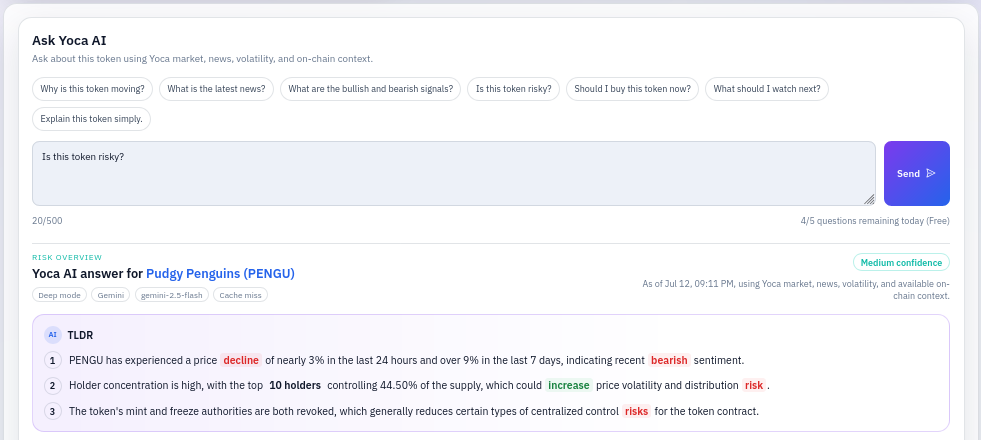
\includegraphics[width=0.88\textwidth]{images/ui/token_overview__ask_yoca_ai_is_this_token_risky.png}

    \vspace{0.4em}
    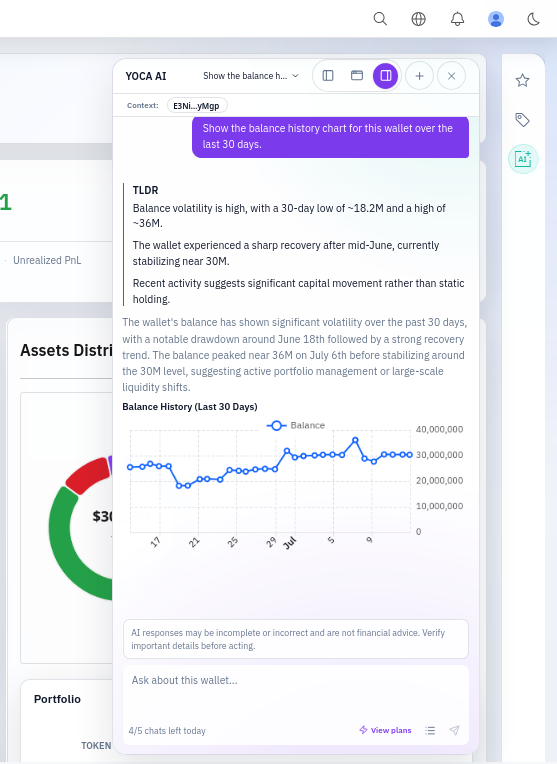
\includegraphics[width=0.46\textwidth]{images/ui/wallet_overview__wallet_ai_histrical_balance_30d.png}
    \caption{Ask Yoca AI phân tích token và Wallet AI giải thích lịch sử số dư 30 ngày}
    \label{fig:yoca-ai-contexts}
\end{figure}

\section{Các giải pháp kỹ thuật tiêu biểu}
\label{sec:giai_quyet_thach_thuc}

\subsection{Điều phối truy vấn và tái sử dụng dữ liệu}

Các provider áp dụng giới hạn theo số request, credit hoặc compute unit. Server đặt yêu cầu sau lớp điều phối theo từng dịch vụ và tái sử dụng dữ liệu đã lưu trước khi gọi ra ngoài. Với dữ liệu snapshot như metadata hoặc market overview, thời điểm cập nhật xác định dữ liệu còn hiệu lực. Với lịch sử giá, số dư, swap và transfer, metadata coverage ghi nhận khoảng đã đồng bộ; khi người dùng mở rộng thời gian, hệ thống chỉ tải phần còn thiếu rồi hợp nhất với dữ liệu trước đó.

Cơ chế này đặc biệt quan trọng với ví có lịch sử dài. Một yêu cầu mới có thể tái sử dụng phần lớn dữ liệu đã tải và chỉ cập nhật đoạn cuối gần thời điểm truy vấn. Các yêu cầu trùng nhau phát sinh đồng thời dùng chung kết quả đang xử lý, hạn chế việc nhiều thành phần giao diện cùng truy vấn một endpoint bên ngoài cho cùng đối tượng.

\subsection{Tổ chức dữ liệu cho phân tích ví}

Phân tích ví cần kết hợp nhiều lớp dữ liệu có ý nghĩa khác nhau. Mobula cung cấp chỉ số PnL, win rate, khối lượng và lịch sử tổng tài sản; Zerion cung cấp lịch sử ở cấp token; Helius cung cấp portfolio, giao dịch chi tiết và sự kiện on-chain. Server chuyển các phản hồi này về mô hình nội bộ, lưu theo địa chỉ cùng kỳ phân tích và cung cấp một contract thống nhất cho giao diện.

PnL tổng hợp phản ánh kết quả giao dịch theo dữ liệu phân tích của provider. Đường biến động theo ngày được xây dựng từ thay đổi tổng tài sản và dòng tiền vào/ra, giúp phân biệt biến động do hiệu quả tài sản với việc người dùng nạp hoặc rút tiền. Lịch sử theo token tiếp tục giữ mức chi tiết cần thiết để giải thích đóng góp của từng vị thế vào kết quả chung.

Helius Enhanced Transactions phục vụ lớp chi tiết giao dịch. Dữ liệu token transfer, native transfer, instruction và account change giúp người dùng đối chiếu hoạt động xuất hiện trong lịch sử swap hoặc transfer. Việc phân tách kết quả tổng hợp và dữ liệu chi tiết giữ cho trang Wallet phản hồi nhanh, đồng thời vẫn cung cấp đường dẫn về giao dịch nguồn.

\subsection{Kiểm soát dữ liệu và kết quả AI}

Phản hồi của provider được kiểm tra bằng schema trước khi đi vào phép tính hoặc cơ sở dữ liệu. Các định danh cốt lõi như token address, wallet address và transaction signature được ràng buộc chặt; metadata bổ sung được xử lý theo khả năng hiện diện của từng nguồn. Lỗi từ dịch vụ bên ngoài được chuyển về nhóm trạng thái thống nhất để giao diện hiển thị loading, empty hoặc error phù hợp.

Đối với AI, hướng dẫn hệ thống được tách khỏi câu hỏi, lịch sử hội thoại và dữ liệu do công cụ trả về. Chỉ những công cụ đã đăng ký mới được gọi; dữ liệu đầu vào được giới hạn theo miền đang phân tích. Mô hình trả kết quả theo cấu trúc xác định, sau đó server kiểm tra nội dung và ánh xạ citation về nguồn đã truy xuất. Nhờ đó, phần diễn giải luôn gắn với token, ví hoặc tập giao dịch đang được người dùng quan sát.

\section{Kết quả kiểm thử và đánh giá}
\label{sec:kiem_thu_danh_gia}

Yoca sử dụng Vitest ở cả client và server. Phía client kết hợp jsdom và Testing Library để kiểm tra component, thao tác người dùng, bảng, biểu đồ, hồ sơ, cảnh báo và thanh toán. Phía server kiểm tra route, service, xác thực, entitlement, payment, webhook, provider mapper, dữ liệu Wallet và các guardrail AI. Fixture và mock tạo ra các trường hợp dữ liệu hợp lệ, dữ liệu rỗng, tham số sai, vượt giới hạn truy vấn và lỗi dịch vụ bên ngoài.

Các test tập trung vào hành vi có khả năng ảnh hưởng trực tiếp đến kết quả hiển thị: kiểm tra ownership của dữ liệu người dùng, chống ghi trùng sự kiện cảnh báo, kết thúc phân trang, chuyển đổi response provider, xử lý trường nullable và từ chối phản hồi AI sai cấu trúc. Zod, hợp đồng TypeScript và ràng buộc PostgreSQL hỗ trợ kiểm tra dữ liệu ở các lớp khác nhau; test xác nhận hành vi khi những lớp này phối hợp trong route hoặc service.

\begin{table}[H]
\centering
\small
\begin{tabularx}{\textwidth}{|L{2.5cm}|C{2.2cm}|C{2.2cm}|X|}
\hline
\textbf{Suite} & \textbf{Test file} & \textbf{Test case} & \textbf{Phạm vi chính} \\
\hline
Client & 16/16 đạt & 178/178 đạt & Component, bảng và biểu đồ, payment, profile, Wallet và Alert History API. \\
\hline
Server & 29/29 đạt & 204/204 đạt & Auth và entitlement, payment, alert/webhook, provider mapping, Wallet, phân trang và AI guardrail. \\
\hline
\end{tabularx}
\caption{Kết quả kiểm thử client và server ngày 12/07/2026}
\label{tab:test_results}
\end{table}

Kết quả trong Bảng~\ref{tab:test_results} cho thấy các luồng nghiệp vụ chính đều có kiểm thử hồi quy và hai suite hoàn tất toàn bộ trường hợp đã định nghĩa. Pipeline CI chạy lại các suite cùng typecheck, lint và production build trước bước triển khai, giúp mỗi revision trên nhánh chính trải qua cùng một quy trình kiểm tra.

\section{Tổng kết chương}
\label{sec:tong_ket_ch4}

Chương 5 đã trình bày quá trình đưa kiến trúc Yoca thành một sản phẩm vận hành trên môi trường triển khai. Các chức năng Market, Token, Pool và Wallet tạo thành luồng phân tích cốt lõi; tài khoản, watchlist và cảnh báo duy trì quá trình theo dõi; Wash Trading và AI bổ sung khả năng phát hiện, trực quan hóa và diễn giải dữ liệu. Những chức năng này được hỗ trợ bởi lớp tích hợp provider, cơ chế tái sử dụng dữ liệu và hợp đồng thống nhất giữa client với server.

Kết quả kiểm thử và triển khai cho thấy hệ thống đáp ứng các nhóm chức năng đã xác định, từ xử lý dữ liệu đến tương tác người dùng. Trên cơ sở đó, Chương 6 tổng kết đóng góp của đề tài và trình bày các hướng mở rộng cho dữ liệu, mô-đun Wash Trading và trải nghiệm phân tích.
